%!TEX encoding = UTF-8 Unicode
%
% Laboratorio di Fisica III
% Esperienza 11
% Anno accademico 2013/2014
% Daniele Brugnara, Alessandro Casalino
%

\documentclass {article}
\usepackage[utf8]{inputenc}
\usepackage{fontenc}
\usepackage[italian]{babel}
\usepackage{graphicx}
\usepackage{float}
\usepackage{fancyhdr}
\usepackage{amsfonts}
\usepackage{amsmath}
\usepackage{amssymb}	
\usepackage{wrapfig}
\usepackage{enumitem}
\usepackage{subfigure}
\usepackage [a4paper, top=1.8cm, bottom=2cm, left=0.9cm, right=0.9cm] {geometry}
\pagestyle{fancy}

% cambiato bottom da 1.8 + logo

\makeatletter
\@addtoreset{section}{part}
\makeatother
\rhead{\LARGE Quaderno di Laboratorio}

\lhead{\large Laboratorio di Fisica IV}
\lfoot{GruppoA10 - A. Casalino}
\cfoot{}
\rfoot{\thepage}
\renewcommand{\headrulewidth}{0.7pt}
\renewcommand{\footrulewidth}{0.7pt}

\begin {document}

\part*{16.09.2014 - Amplificatori Operazionali Ideali}

\section{Introduzione}

In questa sessione di laboratorio abbiamo montato due circuiti con amplificatori operazionali e valutato la loro tensione di output.

\section{Materiali}

\begin{itemize} [noitemsep]
\item Oscilloscopio Agilent DSO-X 2002A (bandwidth $70 MHz$, sample rate $2 GSa/s$);
\item Generatore di tensione continua (max $\pm 25 V$);
\item Generatore di tensione Agilent 33120A con range di frequenza da $100 \mu Hz$ a $15 Mhz$;
\item Multimetro Agilent 34410A (utilizzato come amperometro e per verificare i valori delle resistenze);
\item Un amplificatore operazionale UA741;
\item Resistenze di vari valori;
\item Due capacità da $0.1 \mu F$;
\item Breadboard;
\item Cablaggi vari.
\end{itemize}

\section{Premessa sugli amplificatori operazionali ideali}

Durante l'esperienza valuteremo l'amplificatore operazionale considerandolo come ideale. Infatti, in questa approssimazione (peraltro non eccessivamente limitante visti i valori di corrente in gioco nel nostro caso), valgono (considerando come A e B rispettivamente gli ingressi invertente e non invertente):

\begin{equation}
\Delta V_{AB}=0
\label{eq:regola_V}
\end{equation}
\begin{equation}
I_{AB}=0
\label{eq:regola_I}
\end{equation}

cioè la ddp fra l'ingresso invertente e non invertente è portato ad essere nullo dall'amplificatore operazionale modificando il valore di tensione in output (il cosiddetto \textit{ground virtuale} dato che nei nostri casi l'ingresso non invertente è collegato alla comune del circuito); e la corrente assorbita dall'amplificatore è nulla.
Queste regole verranno utilizzate durante questa sessione per valutare la risposta del circuito a segnali in ingresso, e si intendono utilizzate per tutte le sessioni in cui l'amplificatore è considerato ideale.

\begin{figure}[ht]
 \centering
   {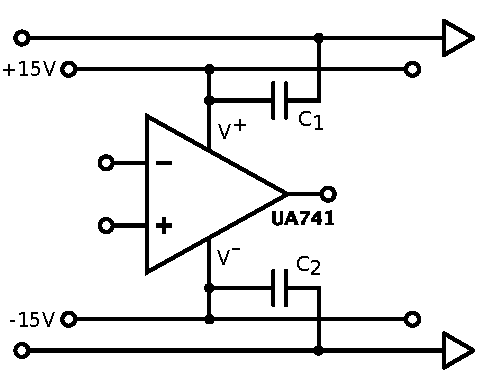
\includegraphics[width=6cm]{alimentazione.pdf}}
 \caption{Grafico dell'alimentazione dell'OPAMP. La tensione di alimentazione è fornita con il generatore di tensione costante, mentre le capacità sono $C_1=C_2=0.1 \mu F$. Per maggiore chiarezza negli schemi circuitali, questa configurazione sarà nascosta negli schemi successivi, ma comunque presente sulla breadboard.}
 \label{gr:costante}
\end{figure}

Inoltre, per maggiore chiarezza degli schemi circuitali, l'amplificatore si intende collegato all'alimentazione ($\pm 15 V$); e, al fine di evitare problemi di noise durante l'alimentazione, abbiamo collegato l'alimentazione a due capacità come nello schema.

\section{Generatore di corrente}

In questo circuito montiamo un generatore di corrente costante, cioè un dispositivo in grado di erogare una corrente costante indipendentemente dal carico a cui è sottoposto. Per valutare la risposta a diverse resistenze di carico abbiamo dunque utilizzato come $R_f$ una resistenza variabile di tipo \textit{trimmer}. Lo schema circuitale è in figura.

\begin{wrapfigure}[21]{r}{0.55\textwidth}
  \begin{center}
    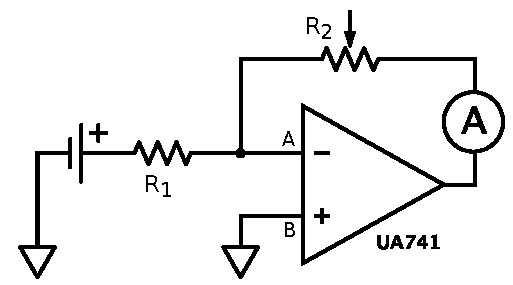
\includegraphics[width=0.40\textwidth]{c1.pdf}
  \end{center}
  \caption{Schema del generatore di corrente costante. Come valori abbiamo utilizzato $R1=3.85 \pm 0.01 k\Omega$ e $V_{gen}=3.85 V$, mentre $R_2$ è variabile. Come amperometro è utilizzato il multimetro, mentre per alimentare l'OPAMP e come generatore di tensione costante in figura, abbiamo utillizzato il generatore di tensione continua.}
\end{wrapfigure}

Risolviamo ora il circuito. Dato che B si trova a potenziale di comune, per (\ref{eq:regola_V}) anche A sarà allo stesso potenziale, che considereremo nullo. Dunque varrà
\begin{equation}
V_{gen}=I R_1
\label{eq:gen_1}
\end{equation}
Per (\ref{eq:regola_I}) e la legge di Kirkhhoff sui nodi, avremo invece che la corrente passante per la resistenza di carico è uguale alla corrente $I$ di (\ref{eq:gen_1}).

Otteniamo dunque che la tensione di output si modificherà, ad opera dell'OPAMP, in modo da far passare sempre lo stesso valore di corrente attraverso $R_2$; ciò avviene per il fenomeno di retroazione negativa, che ci permette di controllare la tensione di output tramite la resistenza di feedback, che in questo caso è proprio $R_2$, e di ottenere dunque una corrente costante passante per il circuito di feedback. Imponendo l'uguaglianza della corrente possiamo inoltre trovare il valore della tensione di uscita
$$V_{out}=\frac{R_2}{R_1} V_{gen}$$

Durante l'esperienza abbiamo però deciso di misurare la corrente passante per la resistenza piuttosto che la tensione di uscita, ponendo un amperometro fra l'uscita dell'OPAMP e la resistenza di carico $R_2$. Come valore di corrente abbiamo scelto $1 mA$ in modo da discostarci dalla corrente massima in cui l'amplificatore operazionale potrebbe non comportarsi più in maniera ideale ($10/20 mA$); e avendo a disposizione una resistenza $R_1=3.85 \pm 0.01 k\Omega$, per (\ref{eq:gen_1}), abbiamo utilizzato una tensione continua di $3.85 V$.

\section{Sommatore Pesato}



\end{document}